

\section*{}
Now a days E-commerce website is very popular in our country. It enables the customers to choose a product or service of their choice from anywhere in the country or the world. Online shops gives us the opportunity to shop 24x7 easily. Just a couple of clicks of the mouse, we can purchase shopping products very easily, which also saves our time. Besides, online shopping allows us to find many products that user wouldn't be able to find in a physical store.\\
Our project named ``Biponee" is an E-Commerce store where there is a vast option of clothing, footwear, jewelry, accessories, electronics, appliance, books, restaurants, health & beauty products etc. We are making this project for an online shop who are currently serving their service by a Facebook page only.\\
%\section{Motivation}


%\label{sec:motivation}  

\section{Project Goal}
The goal of our project is to make it easier to sell product. Customer tracking, online payment system, customer log-in, order management, chatting with customer, cart system, efficient checkout system, promo code system, searching product is the key features of our project.\\
In addition there will be a section in our project where the admins can see the monthly buy and sell report of their shop.
\label{sec:pgoal}



\section{ Project Feasibility Analysis}
  %Feasibilit
  
  \subsection{Technical Feasibility}
  \begin{itemize}
  \item Cost of computers, laptops, printers etc.
  \item Cost of domain, hosting.
  \item Internet quality, availability of internet.
  \item Cost of internet.
  \item 24x7 availability.
  %\newpage
\end{itemize}
%\newpage

  \subsection{Operational Feasibility}
  \begin{itemize}
  \item User Friendly GUI.
  \item Tracking the product.
  \item Monthly buy and sell report.
  \item Chatting system.
  \newpage
  \item Easily add or delete product.
  \end{itemize}
 
   \subsection{ Economical Feasibility}
  \begin{itemize}
  \item Cost of Developers, Programmers etc.
  \item Cost of training the workers to operate with the system.
  \item Cost of Employee for product delivery.
  \end{itemize}
  
   \section{Cost benefit analysis}

 Tangible cost is a quantifiable cost related to an identifiable source or asset. It can be directly connected to a material item used to conduct operations or run any business. Besides  intangible cost is an unquantifiable cost relating to an identifiable source. Intangible costs represent a variety of expenses such as losses in productivity, customer goodwill, loss of brand value or damage to corporate reputation.\\
 \break
 Tangible benefits are those measured in monetary terms and intangible benefits can not be measured in monetary terms but they do have a very significant business impact. 
  
  \begin{table}[h]
  \begin{center}

\begin{tabular}{ |p{5cm}|p{5cm}|p{5cm}|  }

 \hline
  &\textbf{Cost}&\textbf{Benefit}\\
 \hline
\textbf{Tangible}  &-Direct Project Cost &-Making Product order and delivery faster\\
           &-Staff and office space&-Lower inventory cost\\
           &-Implementation Cost&-Improve the rate of productivity\\
           &&-Revenues from advertisers\\
           &&-Improved stock control\\
\hline
\textbf{Intangible}   &-Loss due to server maintenance &-Getting huge number of customers\\
             &-Loss due to training the new employees&-Online payment system\\
             &&-Customer product tracking\\
             &&-Improve Customer satisfaction\\
             &&-Graphical representation of monthly sales report\\
             &&-Improved production scheduling\\
             &&-Rating, 00comment system for customer\\
 \hline

\end{tabular}
\end{center}
\caption{Cost benefit analysis}

%\label{table1}

\end{table}

\newpage

\section{Cash-flow analysis}
Cash flow is the net amount of cash and cash-equivalents being transferred into and out of a business. It is the difference between revenue and total cost of a company. The cash flow analysis is given below:

  \begin{table}[h]
  \begin{center}


\begin{tabular}{ |p{4cm}|p{2.5cm}|p{2.5cm}|p{2.5cm} |p{2.7cm}| }
 \hline
 \multicolumn{5}{|c|}{\textbf{Year 2018}} \\
 \hline
 & \textbf{ Jun-Jul } &   \textbf {Aug-Sept} & \textbf  {Oct-Nov} & \textbf { Dec-Jan }\\
 \hline
 Revenue & 145000 & 232000 & 257000 & 294000\\
 \hline
 Costs &  &  &  & \\
 \hline
 Software Development Cost & 10000  & 10000  & 0 &0 \\
 \hline
 
 Training & 30000  & 35000  & 45000  & 52000 \\
 \hline
 Equipments &  130000 & 150000  & 110000  &  115000\\
 \hline
 Maintain & 0 &  50000 & 82000 & 92000 \\
 \hline
 Total Cost & 170000 & 245000 & 237000  & 259000 \\
 \hline
 Cash Flow & -25000 & -13000  & 20000  & 35000 \\
 \hline
Cumulative Cash Flow & -25000 & -38000  & -18000  & 17000 \\
 \hline
\end{tabular}
\end{center}
\caption{Cash-flow analysis}



\end{table}

\section{Present Value Analysis}
We know that,
\[ P.V=\frac{F.V}{(1+i)^n} \] 

\section*{}
Here,\\
P.V = Present value\\
F.V = Future value\\
i = Interest rate\\
n = Time or period\\
\\
Let us assume that for our project,\\
P.V = 20000\\
n = 4\\
i =0.08\\
So,
\[ F.V={P.V}*{(1+i)^n} \]\\ 
\[ F.V={20000}*{(1+0.08)^4} \]\\ 
\[ F.V=27210 \]\\ 
\newpage

\section{Project Scheduling}
 Project scheduling is a mechanism to communicate what tasks need to get done and which organizational resources will be allocated to complete those tasks in what timeframe. A project schedule is a document collecting all the work needed to deliver the project on time. Our project scheduling is given below: \\
 
 
 \begin{table}[h]
  \begin{center}


\begin{tabular}{ |p{2cm}|p{5cm}|p{3cm}|p{3cm}| }
 \hline
 \textbf{Activity}&\textbf{Description}&\textbf{Predecessors}&\textbf{Time(Days)}\\
 \hline
    A& Project Initiation&None&10\\
 \hline
    B&Report Submission&None&1\\
 \hline
    C&Interview \& Questioning&A, B&7\\
 \hline
    D&Project Planning&C&5\\
 \hline
    E&Analyzing System Needs &C, D&12\\
 \hline
    F&Diagram Designing&E&12\\
    \hline
    G&Data Analysis&C, F&7\\
 \hline
    H&Database Designing&F, G&10\\
\hline
 I&Coding&E, G, H&28\\
 \hline
 J&Documentation&I&5\\
 \hline
K&Testing&I&8\\
\hline
 L&Bug Fixing&K&5\\
\hline
 M&Deployment \& Training&L&10\\
 \hline
\end{tabular}
\end{center}
\caption{Project Scheduling}
\end{table}


\section{Project Scheduling Chart}


\begin{figure}
 
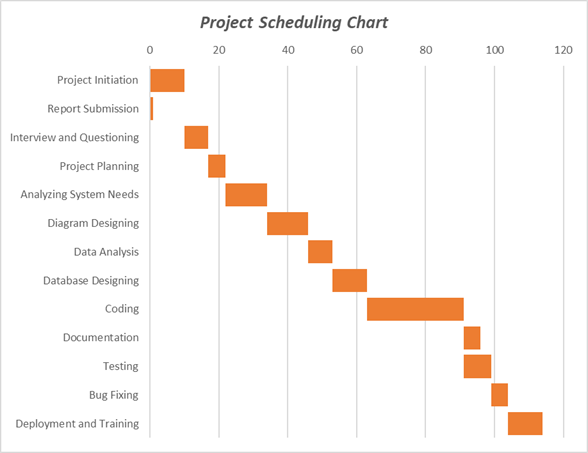
\includegraphics{figures/gantt.png}
\caption{Project Scheduling Chart}
\end{figure}

\newpage


\section{Conclusion}
 Our project ``Biponee" will take around 4 months to complete. After that we submit this project to an E-commerce company. We hope ``Biponee" will contribute a lot to the E-commerce of our country. 













 
 
 






  
